\chapter{Tipos de Sinais}
\label{sinais}

No que tange ao estudo de Circuitos Digitais é muito importante conseguir discernir os tipos de sinais envolvidos. Neste universo os dois principais tipos de sinais são o analógico e o digital. Neste pequeno capítulo vamos apresentar o fundamental destes dois tipos de sinais.


\section{O que é analógico}
\label{sinalAnalogico}

Os sinais presentes na natureza são analógicos. O som, a luz, a temperatura a eletricidade, a pressão, entre outros. 

Cada uma desses fenômenos podem ser sentidos em alguma quantidade. Vamos observar a temperatura (esta observação é valida para todos os outros fenômenos). Imagine um dia de verão - que inicia a uma temperatura de 20,5º e vai \emph{gradativamente} subindo até um pico de 31º, depois retornando a um temperatura menor ao cair da noite.

O que define a temperatura como uma grandeza analógica é a variação gradual entre os valores. Se colocar esta mudança de temperatura em um plano cartesiano (um gráfico), teremos algo que se aproxima de uma curva, que vai subindo até um pico no dia e retorna a um valor mínimo.

O gráfico apresentado na Figura~\ref{fig:temperatura} a seguir demonstra graficamente a variação gradativa da temperatura.

\begin{figure}[h]
	\begin{center}
		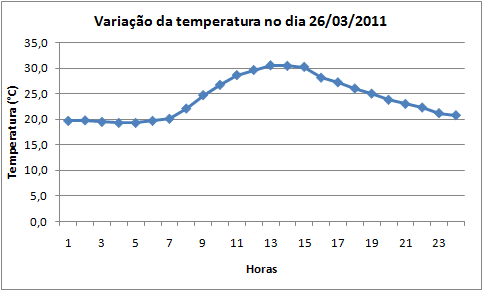
\includegraphics[width=0.85\textwidth]{img/sinais/temperatura.png}
		\caption{Gráfico mostrando a curva de temperatura do dia 26/03/2011.}
		\label{fig:temperatura}
	\end{center}
\end{figure}

Descrição da Figura~\ref{fig:temperatura}:  O gráfico é apresentado em um plano cartesiano. O eixo x representa as horas do dia, iniciando em 1 até 24; o eixo y representa a temperatura iniciando em 0,0 e indo até 35,0 com intervalos de 5. Há linha azul, que demonstra a temperatura do dia - iniciando em 20,0 (das 0h até as 7h)e sobe gradativamente até 31,0 (em torno de 13h) e desce gradativamente até 22,0 (em torno de 23h).


Importante destacar que, se observarmos a linha que descreve a temperatura, em qualquer ponto do gráfico, poderemos perceber que a mudança é gradativa. Em uma definição formal, Tocci (2015) explica que em uma grandeza analógica os valores podem assumir infinitos valores entre um ponto e outro e "... as quantidades podem variar em ao longo de uma faixa contínua de valores...".

Efetivamente, os seres vivos não sobreviveriam, se os fenômenos da natureza não fossem analógicos. A Natureza, e as leis que a regem, criaram um mecanismo compatível com nossas necessidades. É importante que a luz do dia mude gradativamente; o mesmo vale para a temperatura... e também para outras grandezas do nosso planeta. Imaginem se o Sol tivesse uma chave de liga/desliga - ligado é dia, desligado é noite - quais as consequências disso para os seres vivos?

A Figura~\ref{fig:senoide} apresenta uma forma de onda senoidal genérica. Poderia ser usada para representar grandezas de tensão elétrica.

\begin{figure}[h]
	\begin{center}
		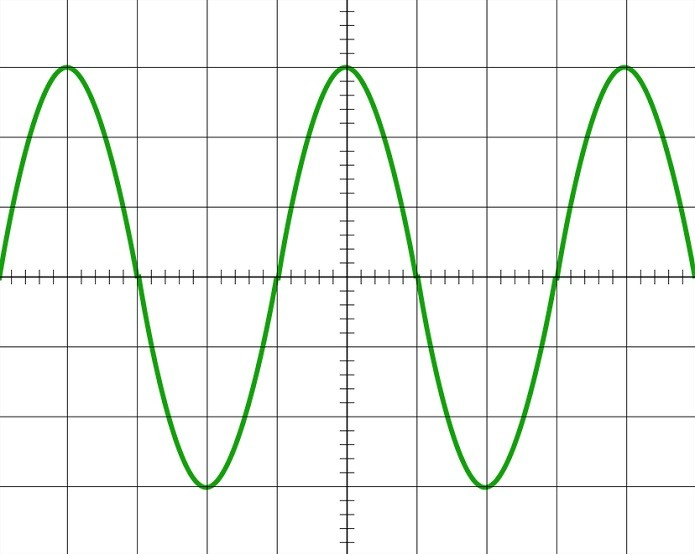
\includegraphics[width=0.85\textwidth]{img/sinais/senoide.png}
		\caption{Gráfico mostrando uma onda senoidal genérico.}
		\label{fig:senoide}
	\end{center}
\end{figure}

Descrição da Figura~\ref{fig:senoide}:  O gráfico contém um plano cartesiano, com eixo X e eixo Y. O eixo x representa a variação do tempo que aumenta para a direita. O eixo y representa a intensidade do sinal que aumenta para cima e diminui para baixo. O sinal representado varia no tempo e na intensidade gradativamente, ou seja, o valor aumenta ou diminui SEM saltos bruscos conforme o tempo passa.


\section{o que é digital}
\label{sinalDigital}

O sinal digital não está presente na natureza, é resultado das criações humanas. Neste tipo de sinal temos uma variação brusca entre dois estados, ou seja, NÃO HÁ variação infinta (ou gradual) entre dois pontos como nos sinais analógicos. 

O exemplo mais comum (e simples de explicar) de sinal digital é a iluminação de uma sala. A lampada está ligada ou desligada - sem estágios intermediários.

Outro sinal bastante simples de explicar é o telegrafo, considerado a primeira foram de comunicação por meio elétrico. Para funcionar, este sistema precisa do código morse, que basicamente é composto por sinais chamados TRAÇO e PONTO. Sendo que ponto é um pulso elétrico de menor duração que o pulso do tipo traço. Este sistema é digital porque consta com dois sinais distintos e únicos - apenas o traço e o ponto. A codificação morse é feita combinando vários destes sinais. 

A Figura~\ref{fig:telegrafo} apresenta os sinais traço/ponto no tempo.

\begin{figure}[h]
	\begin{center}
		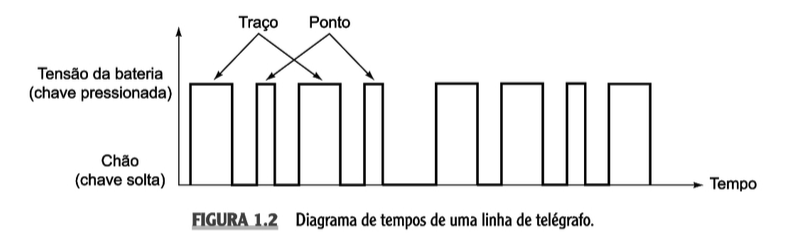
\includegraphics[width=0.85\textwidth]{img/sinais/telegrafo.png}
		\caption{Gráfico mostrando os sinais Traço e Ponto gerados pelo telegrafo. Fonte: Velloso, 2017}
		\label{fig:telegrafo}
	\end{center}
\end{figure}

Descrição da Figura~\ref{fig:telegrafo}: Gráfico de tensão da bateria (eixo Y) por Tempo (eixo X). Tensão alta corresponde a chave do telégrafo pressionada; tensão baixa corresponde a chave do telegrafo solta. Os pulsos gerados são longos (correspondem ao traço) e curtos (correspondem ao ponto).

Formas mais atuais de sinais digitais podem ser explicadas pelo termômetro digital. Este aparelho, usado para medir a temperatura corporal faz a medida de uma grandeza analógica (temperatura do corpo) mas precisa discretizar as medidas para mostrar os valores digitalmente. 

Um termômetro digital comum irá variar a temperatura a cada 0,1 graus C (precisão decimal). Isto quer dizer que valores de temperatura entre o termômetro será capaz de mostrar valores de 36,8 e 36,9. Entretanto o mesmo aparelho não consegue mostrar valores de 36,82 36,83 36,85 - mesmo elas existindo no corpo humano.

O termômetro digital discretiza a amostragem dos valores de temperatura - dando saltos decimais no valor medido. Um tipico termômetro digital é mostrado na Figura~\ref{fig:termometro}

\begin{figure}[h]
	\begin{center}
		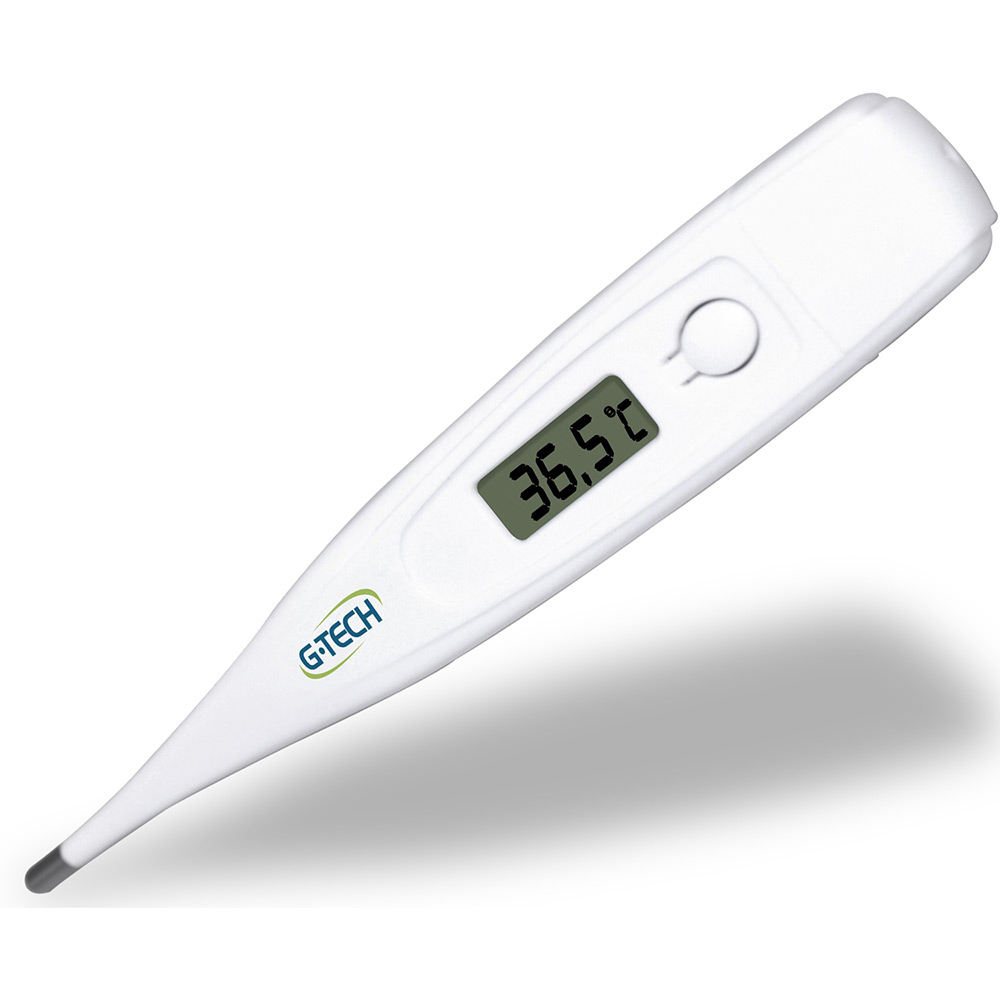
\includegraphics[width=0.85\textwidth]{img/sinais/termometroDigital.png}
		\caption{Um termômetro digital mostrando 36.5 graus C - Fonte: Internet}
		\label{fig:termometro}
	\end{center}
\end{figure}

Ao levar um valor discretizado para um gráfico, teremos uma linha que faz pequenos saltos entre os valores apresentados. Ainda no exemplo do termômetro, que não mostra valores como 31,15 e 31,17, simplesmente o gráfico irá saltar de 31,5 para 31,6. A Figura~\ref{fig:sinaldiscretizado}

\begin{figure}[h]
	\begin{center}
		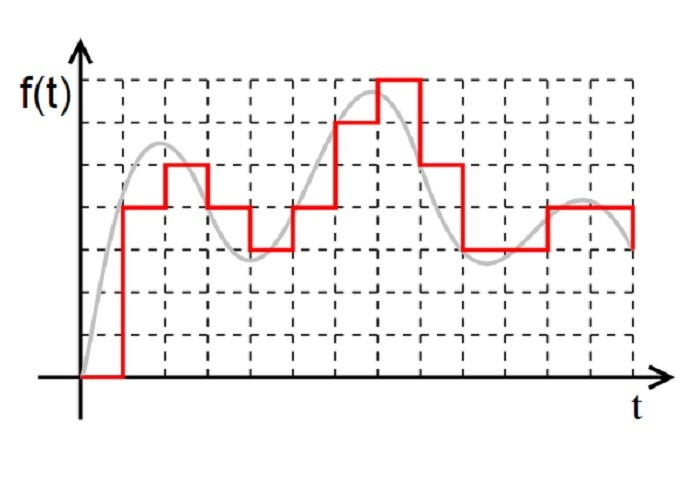
\includegraphics[width=0.85\textwidth]{img/sinais/sinalDiscretizado.png}
		\caption{Um grafio mostrando os saltos entre as medidas de uma grandeza - Fonte: Velloso, 2017.}
		\label{fig:sinaldiscretizado}
	\end{center}
\end{figure}

Descrição da Figura~\ref{fig:sinaldiscretizado}: Gráfico com eixo y, com uma f(t), representando qualquer grandeza, eixo x representando t (Tempo). Duas linhas são desenhadas sobre o gráfico - uma cinza claro que mostra um clássico sinal analógico e sobreposta a esta um linha vermelha demonstrando a discretização - ou seja a linha vermelha tem pequenos saltos entre os valores mostrados "cortando as partes menores".

É muito importante compreender que nossos sentidos não percebem pequenas discretizações. Este problema está presente no exemplo dos discos de música - o disco de vinil é analógico enquanto o CD-ROM é digital. Muitas pessoas alegam que a qualidade sonora da música do vinil é superior a do CD-ROM. Entretanto nossos sentidos (em geral )não são capazes de perceber a diferença. Em outras palavras, a discretização do sinal digital contido no CD-ROM é tão pequena que nossos ouvidos não conseguiriam captar aquele som (mesmo que estivesse presente).

\section{Conversão de sinais}
\label{conversão}

Um problema clássico na área de computação é a conversão entre o mundo digital e o mundo analógico. Para isso vamos analisar a Figura~\ref{fig:conversorAD}. Neste exemplo, trazido por Tocci (2015), temos que controlar a temperatura em um ambiente (poderia ser uma caldeira). O equipamento tem um aquecedor e um sensor. Este ambiente é analógico, mas tudo é controlado por um processador digital (que é digital). O sistema deve ler a temperatura por meio do sensor e controlar (aumentar/reduzir) a temperatura pelo aquecedor. 

Para  isso funcionar, temos dispositivos de conversão entre os mundos analógicos e digitais. No controle do aquecedor, temos um circuito especial que converte comandos digitais do processador para valores analógicos do aquecedor; na leitura do sensor temos um circuito especial que converte o sinal analógico do sensor e e entrega ditalizado para o processador digital.

\begin{figure}[h]
	\begin{center}
		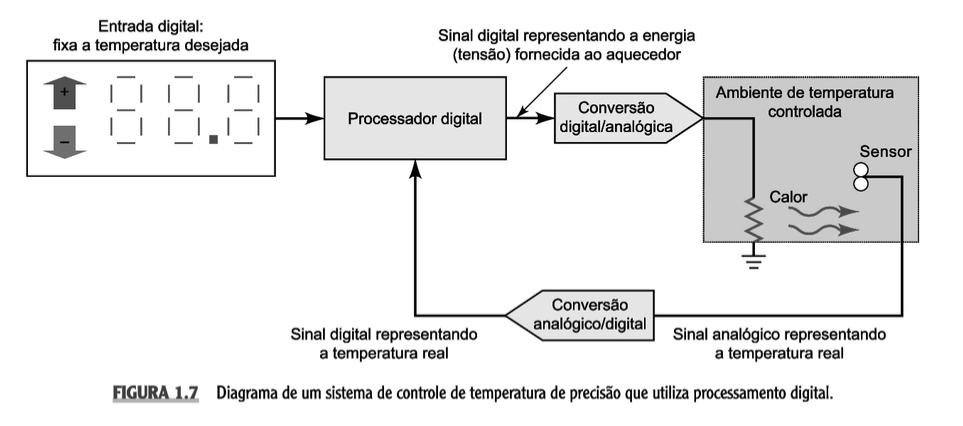
\includegraphics[width=0.85\textwidth]{img/sinais/convertendoSinais.png}
		\caption{Diagrama mostrando um controle digital de caldeira - Fonte: Tocci, 2015.}
		\label{fig:conversorAD}
	\end{center}
\end{figure}

Descrição da Figura~\ref{fig:conversorAD}: A figura apresenta um diagrama de blocos que representa o controle de temperatura em um ambiente. O sistema possui um processador digital, que le um termômetro analógico e controla um aquecedor (também analógico) - tanto aquecedor como sensor estão em uma "caixa". Ligando o processador digital ao aquecedor há um bloco chamado Conversão digital/analógica; e para ligar o sensor de temperatura ao processador digital há um bloco chamado Conversão analógico/digital. Esta figura foi retirada do livro Sistemas Digitais:  Princípios e Aplicações, Tocci, 2015.

\section{Conclusão da seção}

Esse capítulo fez uma breve apresentação sobre os sinais analógicos e digitais. É muito importante que todo estudante de computação tenha uma ciência básica do que os diferencia sinais analógicos de digitais. Importante destacar que há muito mais detalhamentos e aprofundamentos que poderiam ser feitos nessa área de conhecimento. 


\textbf{Bibliografia desta seção:}
Velloso, Felipe. Sinal analógico ou digital? Entenda as tecnologias e suas diferenças. Disponível em <www.techtudo.com.br> Acesso em: Fev 2017.

TOCCI, Ronald J.; WIDMER, Neal S.; MOSS, Gregory L. Sistemas digitais. Pearson Educación, 2010.




